\section{Language Semantics}\label{sec:gr-rules}

Given the graph-based representation of the system state as presented in the previous section, we can now give an operational semantics of the language, by specifying one or more rules for each instruction. Most rules match a certain instruction on top of the continuation stack. Other rules are used for executing sub-routines, e.g. method-lookup.\\
For the specification of such \emph{internal} sub-routines, we choose priorities to help keep the specifications simple. A rule with a certain priority can only be applied when no rule with a higher priority matches. We will use three different priorities. The rules that match base-language instructions have the lowest priority (priority 0). To allow these rules to remove the instruction from the stack, but have sub-routines continue before the next instruction is matched, all base language sub-routine rules have priority 2, i.e. the next instruction continuation stack is matched no sooner than when all sub-routines for the previous instruction have finished. Rules for handling advice have priority 1: they have precedence over base program instructions, but do not interfere with sub-routines. 

\subsection{AFJ semantics}

There are rules for each of the instructions discussed above. However, due to the limited amount of space in this paper, we describe only the rules for the {\sc set}, {\sc call}, and {\sc return} instructions. See \href{http://www.cs.utwente.nl/~staijen/faj/}{http://www.cs.utwente.nl/\~{}staijen/faj/} for the complete set of rules.
%We now describe the rules for the {\sc get}, , , {\sc new},{\sc var}   instruction.

%\paragraph{The {\sc get} and {\sc set} Instructions}
\paragraph{The {\sc set} Instructions}
%Figure \ref{fig:get} shows the graph production rule for the {\sc get} instruction. The rule applies when a \emph{get} instruction is popped from the continuation stack. The get instruction has a {\tt name} edge to a field name in the receiver object. The top of the evaluation stack represents this receiver object. A {\tt Var} node of the receiver object is matched, with the same names as the argument of the {\sc get} instruction. The receiver object is popped from the value stack, and the value of the matched {\tt Var} node is pushed on top of the value stack.

%\begin{figure}
%	\begin{center}
%		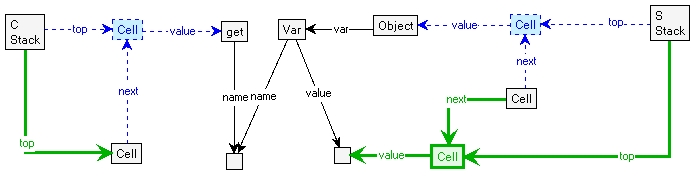
\includegraphics[scale=0.3]{get.png}
%	\end{center}
%		\caption{Rule for the {\sc get} instruction}
%\label{fig:get}
%\end{figure}

Figure \ref{fig:set} shows the rule for the {\sc set} instruction. The rule applies when a {\sc set} instruction is popped from the continuation stack. The receiver object --- containing the field that is to be updated --- is on top of the value stack. The second object on the value stack is the new value of the field. The correct variable  is matched by comparing the identifier attribute of the {\sc set} instruction with the identifiers of the variables in the receiver object. The value of the variable is replaced, and the receiver is popped from the value stack. The assign value remains; it is the result of the expression.

\begin{figure}
	\begin{center}
		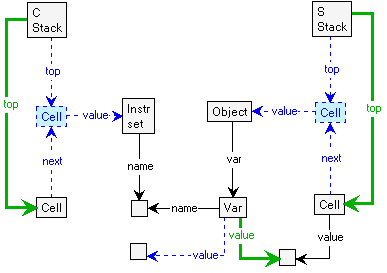
\includegraphics[scale=0.5]{set.png}
	\end{center}
		\caption{Rule for the {\sc set} instruction}
	\label{fig:set}
\end{figure}

\paragraph{The {\sc call} Instruction}

This {\sc call} instruction requires some more work to be done. First, a method-body lookup has to be performed. Second, arguments (that are already on the value stack) have to be transferred to local variables. Third, the instructions of the method-body have to be pushed on top of the continuation stack. To be able to model this, we need to apply a sequence of rules. The entire process of the {\sc call} instruction is described in Figure \ref{lst:call} using pseudo-code.

\begin{figure}[ht]
\begin{lstlisting}[language=Control]
// phase 1: call
call;
// phase 2: method body lookup
until ( call_mbody_match ) do {
  call_mbody_up
}
// phase 3: parameter initialisation
alap { call_initparam }
// phase 4: pushing body on the continuation stack
call_pushcode_start;
until ( call_pushcode_end ) do {
  call_pushcode
}
\end{lstlisting}
\caption{The method-call sub-routine.}
\label{lst:call}
\end{figure}

\begin{figure*}
\centering

\subfigure[\emph{call}]{
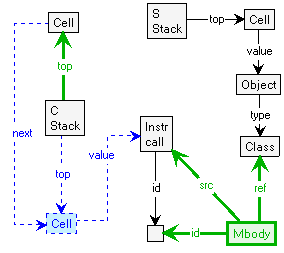
\includegraphics[scale=0.6]{call.png}
\label{fig:subfig1}
}\qquad
\subfigure[\emph{mbody\_match}]{
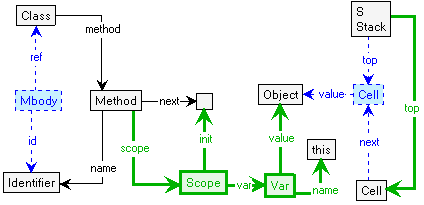
\includegraphics[scale=0.6]{call_mbody_match.png}
}\\
\subfigure[\emph{mbody\_up}] {
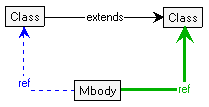
\includegraphics[scale=0.6]{call_mbody_up.png}
}\qquad
\subfigure[\emph{call\_initparam}] {
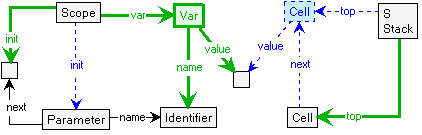
\includegraphics[scale=0.6]{call_initfield.png}
}\\
\subfigure[\emph{call\_pushcode\_start}] {
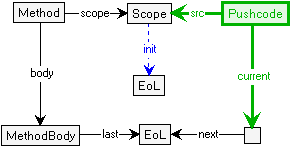
\includegraphics[scale=0.6]{call_pushcode_start.png}
}\qquad
\subfigure[\emph{call\_pushcode}] {
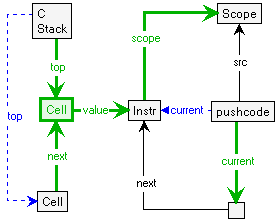
\includegraphics[scale=0.6]{call_pushcode.png}
}\qquad
\subfigure[\emph{call\_pushcode\_end}] {
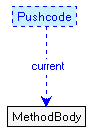
\includegraphics[scale=0.6]{call_pushcode_end.png}
}\\
\caption{The rules for the {\sc call} instruction.}
\label{fig:call_rules}
%{Caption of subfigures \subref{fig:subfig1}, \subref{fig:subfig2} and \subref{fig:subfig3}}
\end{figure*}

The keyword {\tt alap} stand for \emph{as long as possible}, meaning that the mentioned rule is applied until it cannot be matched. The process is divided into four phases. We describe these phase one at a time. The rules for this process are shown in Figure \ref{fig:call_rules}.
\begin{list}{$\bullet$}{}
\item \emph{Phase 1:} A {\sc call} instruction is popped from the continuation stack. The method lookup process is started by creating an {\tt Mbody} node that refers to the type of the receiver object on top of the value stack, and the identifier of the method that is called.
\item \emph{Phase 2:} The {\tt Mbody} searches upwards in the class hierarchy until a method is found with an identifier that matches the associated identifier. When the method is found, a scope is created to contain the variables for the method parameters, and the \emph{this} variable is created with the receiver as value, which is popped from the value stack. An {\tt init} edge is created connecting the scope to the first parameter that is to be initialised.
\item \emph{Phase 3:} As long as the scope has an {\tt init} edge to a Parameter, a value is popped from the value stack and a variable is created storing the value for the parameter. The parameters are initialised in backwards order, consistent with the order of the arguments on the value stack.
\item \emph{Phase 4:} When all parameters have been initialised, a pushcode process is created for pushing the method body on the continuation stack. Each time an instruction is pushed, the {\tt current} edge of the {\tt pushcode} node is updated to the next instruction. The instructions are pushed in reverse order (i.e. starting with the {\sc return} instruction) so that --- when finished --- the first instruction will be on top of the continuation stack.
\end{list}

%\begin{figure}
%	\begin{center}
%		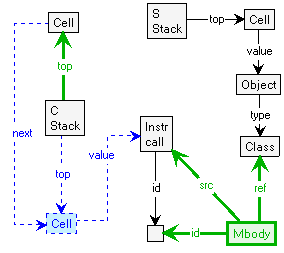
\includegraphics[scale=0.5]{call.png}
%	\end{center}
%		\caption{The \emph{call} rule that matches a call instruction on top of Stack {\tt C}}
%	\label{fig:call}
%\end{figure}

\begin{comment}
Figure \ref{fig:call_mbody_match} and \ref{fig:call_mbody_up} show the rules for the method-lookup.
These rules both match an {\tt mbody} node with a {\tt ref} edge to a {\tt Class} node.
The {\tt call\_mbody\_match} rule has been given a higher priority then {\tt call\_mbody\_up}.
In case the first rule matches, a {\tt Method} node is found in the current "ref" class with the name referred to by the {\tt mbody} node.
Only when no such method is found (i.e. {\tt call\_mbody\_match} does not match) the rule {\tt call\_mbody\_up} will match, updating the {\tt ref} edge of the {\tt mbody} node to the superclass of the current "ref" class. \\
When a matching method is found, a helper node {\tt Scope} is created with an {\tt init} edge to the first parameter of the method, or an {\tt EoL} node.
Also, the {\tt this} reference is created by creating a {\tt Var} node with name {\tt this}, and as value the top of the value stack, which is popped.

\begin{figure}
	\begin{center}
		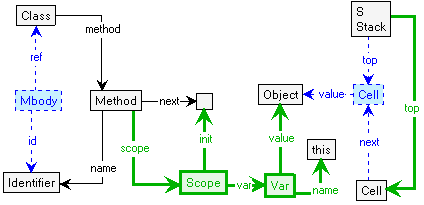
\includegraphics[scale=0.5]{call_mbody_match.png}
	\end{center}
		\caption{The \emph{call\_mbody\_match} rule.}
	\label{fig:call_mbody_match}
\end{figure}

\begin{figure}
	\begin{center}
		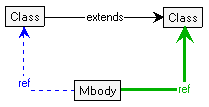
\includegraphics[scale=0.5]{call_mbody_up.png}
	\end{center}
		\caption{The \emph{call\_mbody\_up} rule.}
	\label{fig:call_mbody_up}
\end{figure}

Figure \ref{fig:call_initfield} represents the initialisation of a field. This rule matches when a {\tt Scope} is connected to a {\tt Parameter} by an {\tt init} edge. A value is popped from the value stack and assigned to a newly created {\tt Var} nodes, which is connected to the scope. The {\tt Var} node get the same name as the {\tt Parameter} that is being initialised. The {\tt init} edge is redirected to the next {\tt Parameter}, or {\tt EoL}.

\begin{figure}
	\begin{center}
		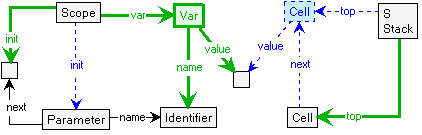
\includegraphics[scale=0.5]{call_initfield.png}
	\end{center}
		\caption{The \emph{call\_initfield} rule.}
	\label{fig:call_initfield}
\end{figure}

Once the {\tt init} edge of the {\tt Scope} node has reached the {\tt EoL} node, initialisation of the parameters is complete. Figure \ref{fig:call_pushcode_start} represents this event, and adds a {\tt pushcode} node to the graph, which triggers the rules that will push the body of the method on the continuation stack. The {\tt pushcode} node receives a {\tt current} edge to the \emph{last} instruction of the method-body. Only for this purpose, this last instruction is connected to the {\tt MethodBody} by a {\tt next} edge.

\begin{figure}
	\begin{center}
		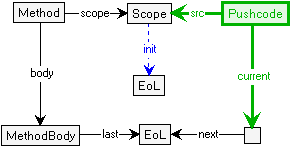
\includegraphics[scale=0.5]{call_pushcode_start.png}
	\end{center}
		\caption{The \emph{call\_pushcode\_start} rule.}
	\label{fig:call_pushcode_start}
\end{figure}

Figure \ref{fig:call_pushcode} shows the \emph{call\_pushcode} rule. This rule matches when the {\tt pushcode} node is connected by a {\tt current} edge to another node. This node is then pushed on top of the continuation stack. The {\tt current} edge is redirected \emph{backwards} over {\tt next} edges; we want to execute the first instruction of the method body first so this instruction should be pushed on top of the continuation stack last.

\begin{figure}
	\begin{center}
		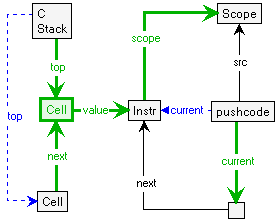
\includegraphics[scale=0.5]{call_pushcode.png}
	\end{center}
		\caption{The \emph{call\_pushcode} rule.}
	\label{fig:call_pushcode}
\end{figure}

Figure \ref{fig:call_pushcode_end} matches when the {\tt current} edge of the {\tt pushcode} node points to the {\tt MethodBody}. The {\tt pushcode} node is deleted ending the process.

\begin{figure}
	\begin{center}
		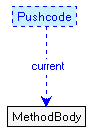
\includegraphics[scale=0.5]{call_pushcode_end.png}
	\end{center}
		\caption{The \emph{call\_pushcode\_end} rule.}
	\label{fig:call_pushcode_end}
\end{figure}

\paragraph{The {\sc new} Instruction}
As mentioned before, a class has no explicit constructor. Instead, when a {\sc new} instruction is executed, the initial values of the class' fields are on the evaluation stack and will be assigned to the corresponding variables of the newly created object. When \emph{new} is finished, the created object is placed on top of the continuation stack.\\
Figure \ref{fig:new} shows the rule that matches the {\tt new} instruction on top of the continuation stack. It creates a new {\tt Object} with a {\tt type} edge to the class and an {\tt init} edge to the first {\tt Field} of the class, or {\tt EoL}. The {\tt init} edge is a triggers the rule for field initialisation.

\begin{figure}
	\begin{center}
		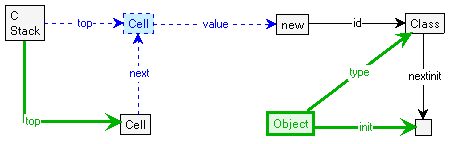
\includegraphics[scale=0.3]{new.png}
	\end{center}
		\caption{The \emph{new} rule.}
	\label{fig:new}
\end{figure}

Figure \ref{fig:new_initfield} shows the rule for the initialisation of a field. It matches when an {\tt Object} node has an {\tt init} edge to a {\tt Field} node. A {\tt Var} node is created and a value is taken from the evaluation stack. The {\tt Var} node is connected to its parent object and the name of the field. The {\tt init} edge is redirected to the next Field (or {\tt EoL}.

\begin{figure}
	\begin{center}
		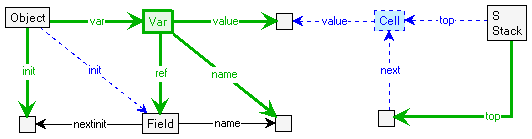
\includegraphics[scale=0.3]{new_initfield.png}
	\end{center}
		\caption{The \emph{new\_initfield} rule.}
	\label{fig:new_initfield}
\end{figure}

Figure \ref{fig:new_end} shows the end of the field initialisation \emph{init} process. This rule is matched when the {\tt init} edge is targeting {\tt EoL} and removes that edge. The new object is pushed on the continuation stack.

\begin{figure}
	\begin{center}
		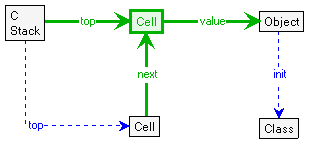
\includegraphics[scale=0.3]{new_end.png}
	\end{center}
		\caption{The \emph{new\_end} rule.}
	\label{fig:new_end}
\end{figure}

%Currently, it is unspecified how inherited fields are handled during initialisation.  For now we let every class also have fields that are specified in the superclass.

\end{comment}

\paragraph{The {\sc return} Instruction}

Due to the sequentialisation defined in Figure \ref{fig:fja_restack}, every method body ends with a {\sc return} instruction. It cleans up any run-time information regarding method-execution. The corresponding graph production rule is shown in Figure \ref{fig:return}. The {\tt Scope} that was created during execution of the {\sc call} instruction is deleted.\\
\\

\begin{figure}
	\begin{center}
		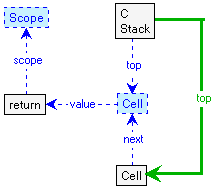
\includegraphics[scale=0.5]{return.png}
	\end{center}
		\caption{The \emph{return} rule.}
	\label{fig:return}
\end{figure}

\begin{comment}

\paragraph{The {\sc var} Instruction}
Figure \ref{fig:var} shows the \emph{var} rule. A {\sc var} instruction --- not to be confused with a class field access using the get instruction --- is the usage of a method argument. When the {\sc var} instruction referring to a variable name is on top of the continuation stack, the rule will match the {\tt Var} node in its scope that has that same name. The resulting value is pushed on the evaluation stack. 

\begin{figure}
	\begin{center}
		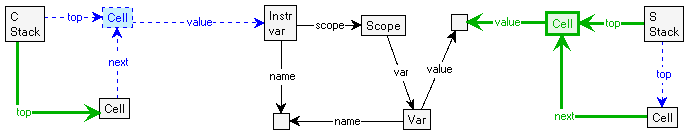
\includegraphics[scale=0.3]{var.png}
	\end{center}
		\caption{The \emph{var} rule.}
	\label{fig:var}
\end{figure}

\end{comment}

\subsection{FAJ Semantics}\label{sec:gr-aspects}

\begin{figure}
\centering
\subfigure[Start state]{
\qquad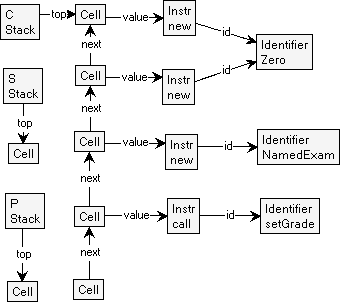
\includegraphics[scale=0.4]{examples/startstate.png}\qquad
\label{fig:state1}
}\\
\subfigure[After scheduling advices]{
\qquad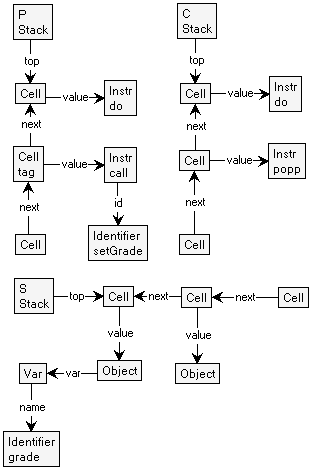
\includegraphics[scale=0.4]{examples/after_both_around.png}\qquad
\label{fig:state2}
}\\
\subfigure[After first proceed]{
\qquad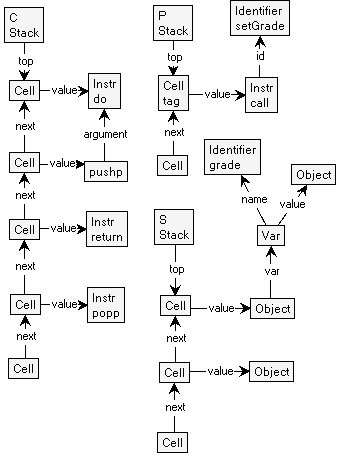
\includegraphics[scale=0.4]{examples/after_first_proceed.png}\qquad
}
\caption{Run-time part of Three States}
\label{fig:example-states}
\end{figure}


When an instruction is on top of the continuation stack and is matched by one or more point-cuts, the associated advices are scheduled by pushing the {\sc do} instructions (linking the point-cuts with the advices) on (a) the continuation stack, if the advice is scheduled first; (b) the proceed stack if the advice is scheduled after the first advice. The original instruction is popped from the continuation stack and pushed on the proceed stack. The {\sc do} instruction invokes the advice, by starting the parameter initialisation and pushcode process, identically as described above for to the {\sc call} instruction. When a {\sc proceed} instruction is executed, the top of the proceed stack is pushed back on the continuation stack. To not have this instruction trigger advice again, the instruction is \emph{tagged}; a tagged instruction can not trigger advice. To handle advice without a {\sc proceed} instruction, when the advices are scheduled, a {\sc popp} instruction is pushed on the continuation stack first. After executing the advices, this instruction pops any remaining instructions for the join point from the proceed stack. For the {\sc popp} instruction to be able to function (it must pop at least one instruction), the proceed rule pushes a {\sc pushp} instruction on the continuation stack, that, after returning from the proceeded instruction, pushes this instruction back on the proceed stack, where it will then immediately be popped from by the {\sc popp} instruction.\\
\\
To illustrate the mechanism of advice execution, we explain the content of the stacks in a number of stages in the execution of the second example scenario. The figures are shown in Figure \ref{fig:example-states}: 
\begin{list}{$\bullet$}{}
\item \emph{(a). Initial state}:  The continuation stack $C$ contains the main expression (see Fig. \ref{fig:example} line 28), which is sequentialised into: {\sc new}$_{Zero}$; {\sc new}$_{Zero}$;{\sc new}$_{NamedExam}$; {\sc call}$_{setGrade}$. Stack $P$ and $S$ are empty.
\item \emph{(b). After the two advices are scheduled}: The $S$ stack contains the {\tt Zero} object and the {\tt NamedExam} object, with the {\tt Var} representing grade zero. The continuation stack contains, from top to bottom: a {\sc do} instruction that will invoke the first advice; a {\sc popp} that pops any remaining instructions for the join point from the proceed stack. The proceed stack contains, from top to bottom: a {\sc do} instruction for the second advice, such that proceed in the first advice will execute the second advice; the tagged {\sc call} instruction for {\tt setGrade}, that will be executed by proceed in the second advice.
\item \emph{(c). After the first {\sc proceed} instruction}: Since proceed is called on the initial receiver of the intercepted {\sc call}, and has the arguments of the intercepted call as arguments, the $S$ stack has not changed w.r.t. previously described state. The proceed stack now contains only the {\sc call} instruction that triggered the advices. The continuation stack contains, from top to bottom: the {\sc do} instruction that will invoke the second advice; a {\sc pushp} instruction that will push the {\sc do} instruction back on the proceed stack (after the advice has returned); the {\sc return} instruction of the first advice; and the {\sc popp} instruction that will clean up the proceed stack.\\
\end{list}

The most important rules are displayed in Figure \ref{fig:aspect_rules}. The \emph{around} rule takes care of the first advice that is scheduled and creates a join point instance. This instance is used to trigger matching any subsequent advices that, instead of matching an instruction on the continuation stack, match an instruction on the proceed stack referred to by this join point. The neglected rules can be found at See \href{http://www.cs.utwente.nl/~staijen/faj/}{http://www.cs.utwente.nl/\~{}staijen/faj/}. 

\begin{figure*}[ht]
\centering
\subfigure[\emph{around}]{
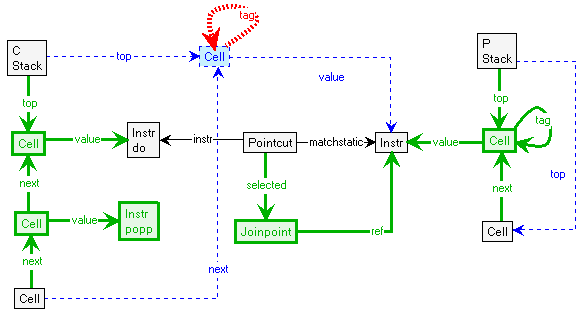
\includegraphics[scale=0.45]{aspect/around.png}
}\\
\subfigure[\emph{proceed}]{
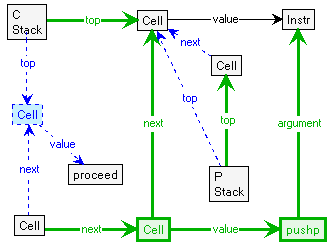
\includegraphics[scale=0.45]{aspect/proceed.png}
}\qquad\qquad
\subfigure[\emph{do}] {
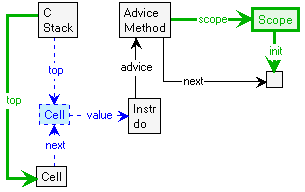
\includegraphics[scale=0.45]{aspect/do.png}
}
\caption{The Rules for Advice Execution.}
\label{fig:aspect_rules}
%{Caption of subfigures \subref{fig:subfig1}, \subref{fig:subfig2} and \subref{fig:subfig3}}
\end{figure*}

%Whenever a point-cut matches an instruction on top of the continuation stack, the system will execute the advice code before the matched instruction is executed. This is model;ed in such a way that, for any number of advice triggered by an instruction, each of these advice can be handled in a uniform way. 

%The \emph{around} rule will query the environment for any advice matching the instruction statically, and will push a {\sc test} instruction for the first advice on top of the continuation stack, together with a {\sc popp} instruction (which is positioned under the test instruction) that pops all remaining instructions for the join-point from the proceed stack. This instruction is needed in case there is no proceed in an advice body. The original instruction is moved to the top of the proceed stack.\\
%Then for every next advice, a test instruction is pushed on the proceed stack P. The initial instruction is \emph{tagged}; tagged instructions can not trigger advice. The \emph{proceed} rule will pop an element from the proceed stack on push it on the continuation stack, together with another instruction afterwards to push the instruction back on the proceed stack.\\
%We will clarify this process in more detail by describing the rules that are involved.

\begin{comment}

\begin{figure}
	\begin{center}
		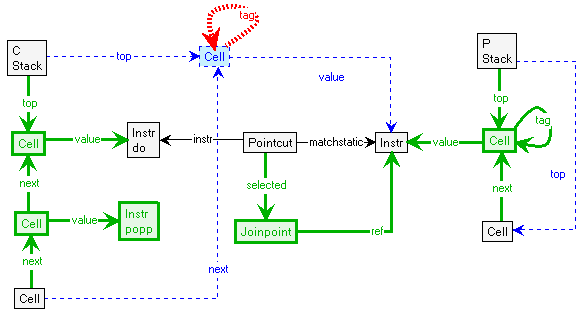
\includegraphics[scale=0.3]{aspect/around.png}
	\end{center}
		\caption{The \emph{around} rule}
	\label{fig:around}
\end{figure}

Figure \ref{fig:around} shows the graph production rule \emph{around}. A instruction statically matched by a point-cut is on top of the continuation stack. The instruction is popped from the continuation stack and pushed on top of the proceed stack. Since instructions are static elements, we cannot tag the instruction itself; it would still be tagged the next time it is scheduled to be executed. Therefore, the {\tt Cell} is tagged. The \emph{around} rule only matches when the cell was not tagged yet. This is specified by \emph{tag} NAC.\\
A new {\tt test} instruction is created and placed on top of the continuation stack. A {\tt popp} instruction is placed right under the test instruction.\\
Subsequent advices (on the same join point) have to be matched differently, since the instruction is no longer on the continuation stack. This has been dealt with, but we do not elaborate on that in this paper.

\begin{figure}
	\begin{center}
		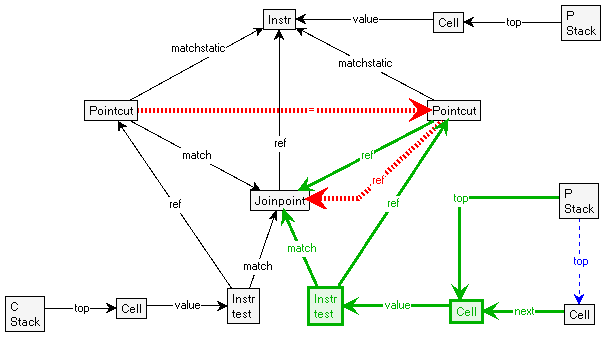
\includegraphics[scale=0.3]{aspect/around_more.png}
	\end{center}
		\caption{The \emph{around\_more} rule}
	\label{fig:around_more}
\end{figure}

Figure \ref{fig:around_more} shows the rule that is required to handle more than one advice. Because the advice-triggering instruction was pushed on the proceed stack by the first advice, instead of matching an instruction on the continuation stack, the rule matches an instruction on the proceed stack that is referred to by a {\tt Joinpoint}. This rule does not require the instruction to be untagged; it was tagged by the rule matching the first advice. The rule only matches point-cuts that have no {\tt ref} edge to the {\tt Joinpoint} node yet and, when applied, the rule adds this edge to the selected point-cut. 

\begin{comment}
\begin{figure}
	\begin{center}
		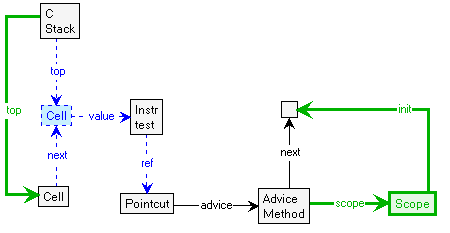
\includegraphics[scale=0.5]{aspect/test.png}
	\end{center}
		\caption{The \emph{test} rule}
	\label{fig:test}
\end{figure}

The test instruction is meant for dynamic matching of point-cuts. We have included this instruction in our model but have not specified any dynamic tests. Therefore, the test instruction will always perform a positive point-cut match, and schedule the advice for execution. The rule for the {\sc test} instruction is shown in Figure \ref{fig:test}. The instruction is popped from the continuation stack. Notice that the instruction is not deleted; this is because it will be pushed by pushp afterwards in case it was put in the continuation stack by an application of the \emph{proceed} rule. The \emph{pushcode} process is started to put the advice on the continuation stack.

\begin{figure}
	\begin{center}
		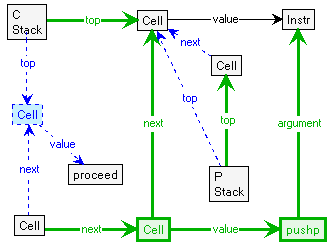
\includegraphics[scale=0.3]{aspect/proceed.png}
	\end{center}
		\caption{The \emph{proceed} rule}
	\label{fig:proceed}
\end{figure}

Figure \ref{fig:proceed} shows the graph production rule for the {\sc proceed} instruction. It matches a proceed instruction on top of the continuation stack, which is popped. The top of the proceed stack is popped and pushed on top of the continuation stack, together with a newly created \emph{pushp} instruction, which has the a {\tt argument} edge to the instruction that is to be pushed.\\

\begin{figure}
	\begin{center}
		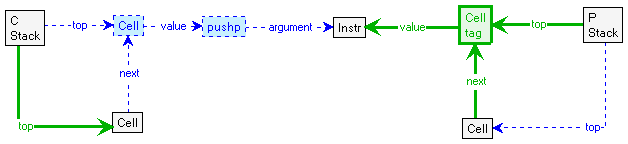
\includegraphics[scale=0.3]{aspect/pushp.png}
	\end{center}
		\caption{The \emph{pushp} rule}
	\label{fig:pushp}
\end{figure}

Figure \ref{fig:pushp} shows the graph production rule for the {\sc pushp} instruction. It pops the pushp instruction from the continuation stack and pushed its argument, an instruction, on top of the proceed stack.

\begin{figure}
	\begin{center}
		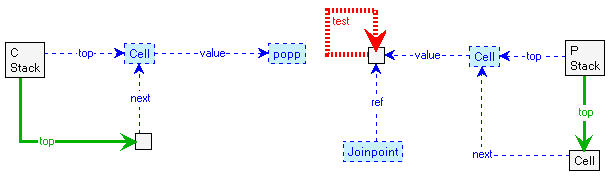
\includegraphics[scale=0.3]{aspect/pop.png}
	\end{center}
		\caption{The \emph{popp} rule}
			\label{fig:pop}
\end{figure}

Figure \ref{fig:pop} shows the rule for the {\sc popp} instruction. This rule matches a popp instruction on the continuation stack and also pops this instruction. An instruction is popped from the proceed stack. However, the instruction is not deleted since it is part of our static environment. The rule does not match test instructions on the proceed stack since these are treated differently. 

\begin{figure}
	\begin{center}
		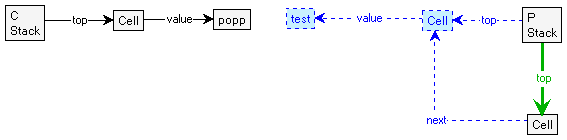
\includegraphics[scale=0.3]{aspect/pop_test.png}
	\end{center}
\caption{The \emph{pop\_test} rule}
	\label{fig:pop_test}
\end{figure}

Figure \ref{fig:pop_test} shows the rule for the {\sc popp} instruction and a test instruction is on top of the proceed stack. In this case, the test instruction is deleted, since this instruction is not part of our environment, but was created just for the purpose of being able to match advice dynamically. When dealing with multiple advice, after all advice have executed, the proceed stack will contain a sequence of test instructions followed by the triggering instruction. All test instructions are popped by leaving the popp instruction on the continuation stack until the static instruction is popped, i.e. when the rule in Figure \ref{fig:pop} is applied.\\

One last rule is required to model advice. Advice is modelled as a method body. A regular return instruction in a method body pops the call from the call stack. Advice, however, is not pushed on the call stack, and should thus also not be popped. Figure \ref{fig:advice_return} shows the \emph{advice\_return} rule. It matches a {\tt return} instruction on top of the continuation stack, that is the last instruction of the body of an advice. The {\tt Scope} is deleted and the instruction is popped. No {\tt call} instruction is popped from the call stack.

\begin{figure}
	\begin{center}
		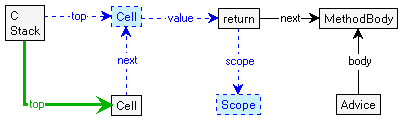
\includegraphics[scale=0.3]{aspect/advice_return.png}
	\end{center}
		\caption{The \emph{advice\_return} rule}
	\label{fig:advice_return}
\end{figure}
\end{comment}
